\documentclass[handout]{beamer}

\usepackage{Haust2017glærur}

\title{Stærðfræðimynstur í tölvunarfræði}
\subtitle{Vika 9, fyrri fyrirlestur}

\begin{document}

\begin{frame}
\titlepage
\end{frame}


\section{Inngangur}

\begin{frame}{Í síðasta tíma}
    \begin{itemize}
        \item N-undarvensl og gagnagrunnar
        \item Venslaaðgerðir
        \item Framsetning vensla með fylkjum
        \item Netaframsetning á venslum
    \end{itemize}
\end{frame}

\section{Rakningarvensl - upprifjun}

\begin{frame}{Rakningarvensl}
\begin{tcolorbox}[title=Rakningarvensl]
Rakningarvensl (e. \emph{recurrence relation}) fyrir runu $\{a_n\}$ er jafna sem skilgreinir $a_n$ sem fall af einum eða fleiri fyrri liðum rununnar, þ.e.a.s. $a_0, a_1, \ldots, a_{n-1}$ fyrir öll $n > n_0$, þar sem $n_0$ er ekki-neikvæð heiltala.
\end{tcolorbox}
Runa er lausn (e. \emph{solution}) á rakningarvenslum ef liðir hennar uppfylla venslin. Liðirnir sem eru fyrir framan fyrsta liðinn sem rankningarvenslin tilgreina eru upphafsskilyrði (e. \emph{initial conditions}) þeirra.
\end{frame}

\begin{frame}{Dæmi um rakningarvensl}
Látum $\{a_n\}$ vera runu sem uppfyllir $a_n = a_{n-1} + 3$ fyrir $n=1, 2, 3, \ldots$ og setjum $a_0 = 2$. Hvað eru þá $a_1, a_2$ og $a_3$? \pause

\begin{align*}
a_1 &= a_0 + 3 = 2 + 3 = 5\\
a_2 &= 5 + 3 = 8\\
a_3 &= 8 + 3 = 11\\
\end{align*}

\end{frame}

\begin{frame}{Dæmi um rakningarvensl}
\begin{itemize}
 \item Fibonacci-rununa $f_0, f_1, f_2, \ldots$ má skilgreina með rakningarvenslum
 \begin{itemize}
  \item Upphafsskilyrði: $f_0 = 0, f_1 = 1$
  \item Rakningarvensl: $f_n = f_{n-1} + f_{n-2}$
 \end{itemize}
\end{itemize}
\end{frame}

\section{Endurkvæmni}

\begin{frame}{Endurkvæm lýsing á föllum}
\begin{itemize}
 \item Rakningarvensl eru runur þar sem seinni liðir eru skilgreindir út frá fyrri liðum
 \item Hægt er að nota endurkvæmni (e. \emph{recursion}) til að skilgreina föll út frá sjálfum sér
 \item Endurkvæm skilgreining á falli (með mengi ekki-neikvæðu heiltalnanna sem formengi) fer fram í tvennu lagi:
 \begin{enumerate}
  \item Grunnskref (e. \emph{basis step}) skilgreinir fallsgildi fallsins í núlli eða nálægt núlli
  \item Endurkvæmt skref (e. \emph{recursive step}) gefur reglu til að finna fallsgildi fallsins í gefinni heiltölu með því að nota gildi fallsins af lægri heiltölum
 \end{enumerate}
 \item Endurkvæmni er líka kölluð rakning, endurkvæma skrefið er líka kallað þrepunarskref (e. \emph{inductive step})
\end{itemize}
\end{frame}

\begin{frame}{Endurkvæmt fall}
Við getum skilgreint fall á eftirfarandi hátt:
\begin{align*}
f(0) &= 3\\
f(n+1) &= 2f(n) + 3
\end{align*}
Hvernig finnum við gildi $f(4)$? \pause Finnum öll minni fallsgildi, og reiknum:
\begin{align*}
f(1) = 2f(0) + 3 &= 2 \cdot 3 + 3 = 9\\
f(2) = 2f(1) + 3 &= 2 \cdot 9 + 3 = 21\\
f(3) = 2f(2) + 3 &= 2 \cdot 21 + 3 = 45\\
f(4) = 2f(3) + 3 &= 2 \cdot 45 + 3 = 93
\end{align*}
\end{frame}

\begin{frame}{Endurkvæm skilgreining}
Hvernig getum við á endurkvæman máta skilgreint stærðina $a^n$, þar sem $a$ er rauntala önnur en $0$ og $n$ er jákvæð heiltala?
\pause
\begin{itemize}
 \item Grunnskref: Skilgreinum $a^0 = 1$.
 \item Endurkvæmt skref: $a^{n+1} = a \cdot a^n$
\end{itemize}
\end{frame}

\section{Endurkvæm skilgreining mengja}

\begin{frame}{Endurkvæm skilgreining mengja}
\begin{itemize}
 \item Hægt er að skilgreina mengi á endurkvæman máta 
 \begin{itemize}
  \item Grunnskref: Tilgreinum safn staka sem tilheyrir menginu
  \item Endurkvæmt skref: Tilgreinum reglu til að búa til ný stök út frá upphaflegu stökunum
 \end{itemize}
\end{itemize}
\end{frame}

\begin{frame}{Endurkvæm skilgreining}
\begin{itemize}
 \item Skilgreinum $S$, mengi allra jákvæðra margfelda af $3$:
 \begin{itemize}
  \item Grunnskref: $3 \in S$
  \item Endurkvæmt skref: Sé $x \in S$ og $y \in S$, þá er $x+y \in S$
 \end{itemize}
\end{itemize}
\end{frame}

\begin{frame}[fragile]{Upprifjun - Strengir}
\begin{itemize}
 \item Sérstök, mikið notuð gerð af runum kallast strengur (e. \emph{string})
 \item Strengur er endanleg runa af stöfum, úr endanlegu mengi (stafrófinu)
 \begin{itemize}
  \item Stafrófið getur verið hvaða mengi sem er, en algeng stafróf eru \texttt{\{'a', 'b', 'c', \ldots\}} og \texttt{\{0, 1\}}
 \end{itemize}
 \item Strengur með engum stöfum (af lengdinni $0$) er kallaður tómur og táknaður með $\lambda$
\end{itemize}
\end{frame}

\begin{frame}{Strengir - endurkvæm skilgreining}
\begin{itemize}
 \item Við getum skilgreint mengi strengja $\Sigma^*$ yfir stafrófið $\Sigma$ á endurkvæman hátt:
 \begin{itemize}
  \item Grunnskref: $\lambda \in \Sigma^*$
  \item Endurkvæmt Skref: Sé $w \in \Sigma^*$ og $x \in \Sigma$, þá er $wx \in \Sigma^*$
 \end{itemize}
 \item Þ.e.a.s. ef við skeytum staf úr stafrófinu aftan á streng fáum við annan streng
\end{itemize}
\end{frame}

\begin{frame}{Strengjasamskeyting}
\begin{itemize}
 \item Getum skilgreint samskeytingu (e. \emph{concatenation}) tveggja strengja á endurkvæman átt:
 \begin{itemize}
  \item Grunnskref: Sé $w \in \Sigma^*$ er $w\lambda = w$
  \item Endurkvæmt Skref: Sé $w_1 \in \Sigma^*$ og $w_2 \in \Sigma^*$ og $x \in \Sigma$, þá er $w_1(w_2x) = (w_1w_2)x$
 \end{itemize}
 \item Dæmi: Sé $w_1 = abra$ og $w_2 = cadabra$ er $w_1w_2 = abracadabra$.
\end{itemize}
\end{frame}

\section{Endurkvæm reiknirit}

\begin{frame}{Endurkvæm reiknirit}
\begin{itemize}
 \item Munum að reiknirit er endanleg runa vel skilgreindra aðgerða sem reikna út lausn á skilgreindu vandamáli
 \item Reiknirit hefur inntak, sem lýsir tilviki af vandamálinu sem það leysir
 \item Reiknirit er kallað endurkvæmt ef það leysir vandamálið með því að smætta það niður í smærra tilvik af sama vandamáli
\end{itemize}
\end{frame}

\begin{frame}{Endurkvæmt hrópmerkt}
Hrópmerkt hentar vel til endurkvæms útreiknings.
\begin{center}
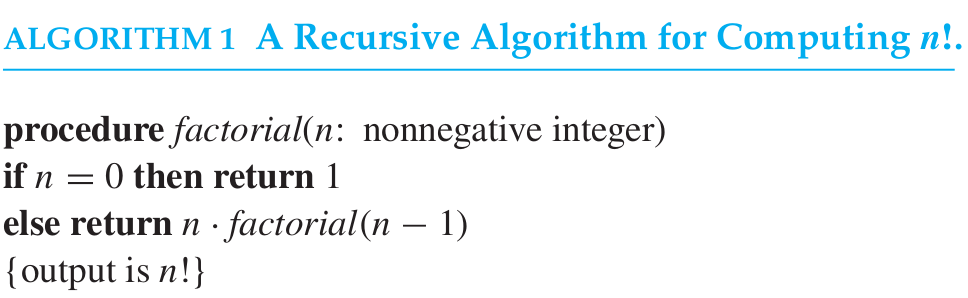
\includegraphics[width=\textwidth]{factorial-algorithm}
\end{center}
\pause
\[
3! = 3\cdot 2! = 3 \cdot 2 \cdot 1! = 3 \cdot 2 \cdot 1 \cdot 0! = 3 \cdot 2 \cdot 1 \cdot 1
\]
\end{frame}

\begin{frame}{Endurkvæmt GCD}
\begin{columns}
\column{0.5\textwidth}
Við getum reiknað stærsta samdeili (gcd) með endurkvæmu reikniriti sem byggir á því að 
\[
 gcd(a,b) = gcd(b \Mod a, a)
\]
og að 
\[
 gcd(0,b) = b
\]
þegar $b > 0$.
\column{0.5\textwidth}

\vspace{0.5cm}
Þannig getum við reiknað stærsta samdeili 5 og 8:
\begin{align*}
gcd(5,8) &= gcd(8 \Mod 5, 5)\\
&= gcd(3,5)\\
&= gcd(5 \Mod 3, 3)\\
&= gcd(2,3)\\
&= gcd(3 \Mod 2, 2)\\
&= gcd(1,2)\\
&= gcd(2 \Mod 1, 1)\\
&= gcd(0,1)\\
&= 1
\end{align*}

\end{columns}
\end{frame}

\begin{frame}{Endurkvæmt GCD}
Við getum skrifað reiknirit út frá þessari innsýn:
\begin{center}
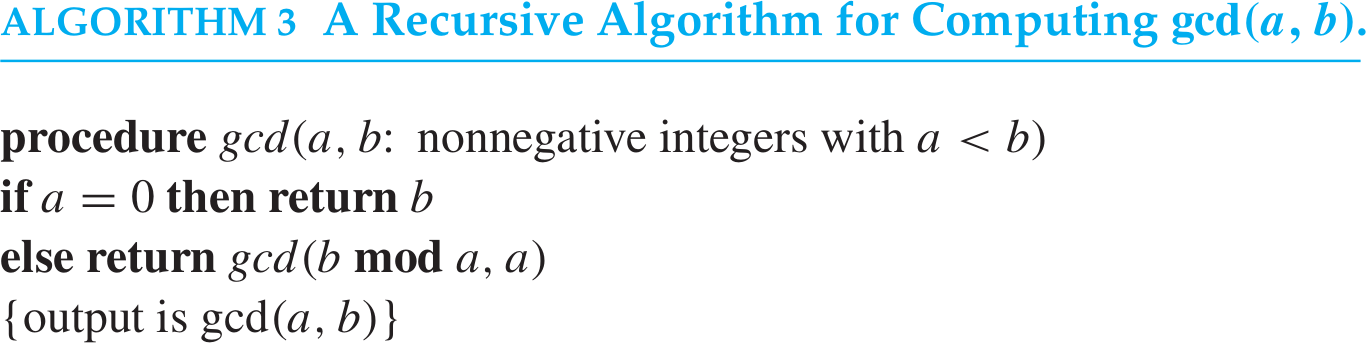
\includegraphics[width=\textwidth]{gcd-recursive}
\end{center}
\end{frame}

\begin{frame}{Línuleg leit}
Rifjum upp línulega leit:
\begin{center}
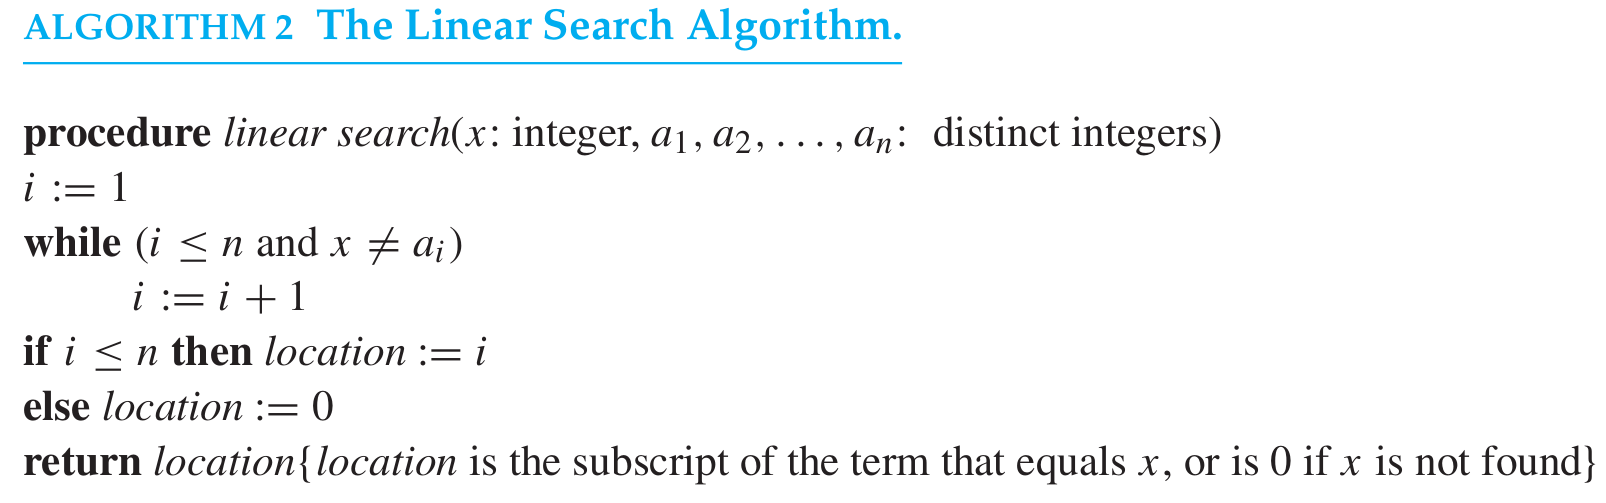
\includegraphics[width=\textwidth]{linear-search}
\end{center}
\end{frame}

\begin{frame}{Endurkvæm línuleg leit?}
Getum við gert endurkvæma útgáfu af línulegri leit?\pause

Já, við getum það:
\begin{center}
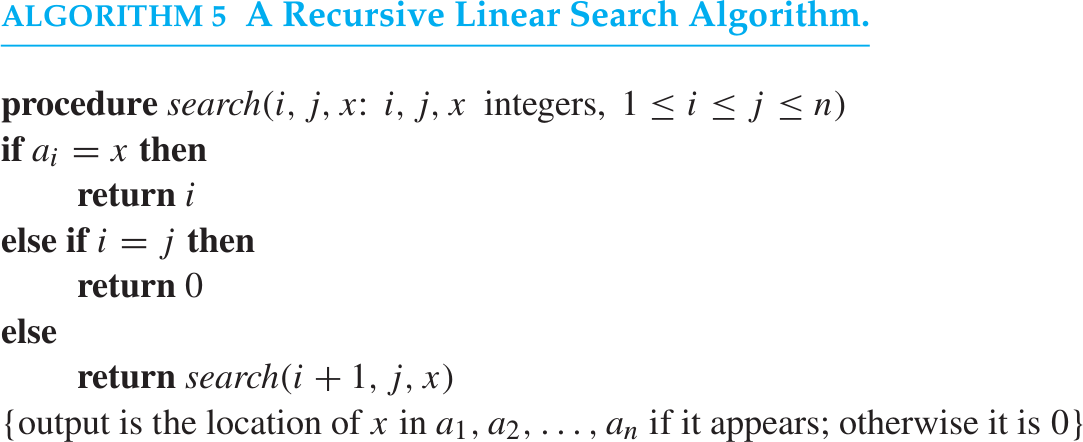
\includegraphics[width=\textwidth]{linear-search-recursive}
\end{center}
\end{frame}

\begin{frame}{Helmingunarleit}
Rifjum upp helmingunarleit:
\begin{center}
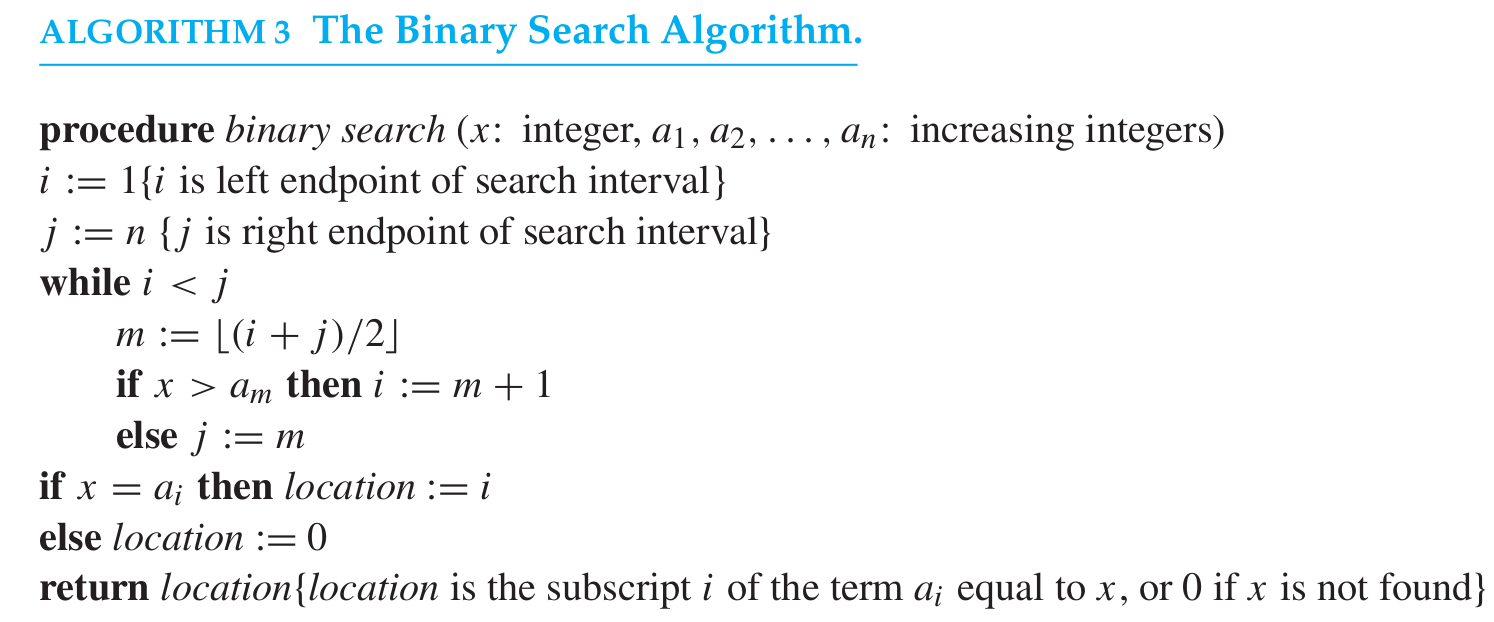
\includegraphics[width=\textwidth]{binary-search}
\end{center}
\end{frame}

\begin{frame}{Endurkvæm helmingunarleit?}
Getum við gert endurkvæma útgáfu af helmingunarleit?\pause

Já, við getum það:
\begin{center}
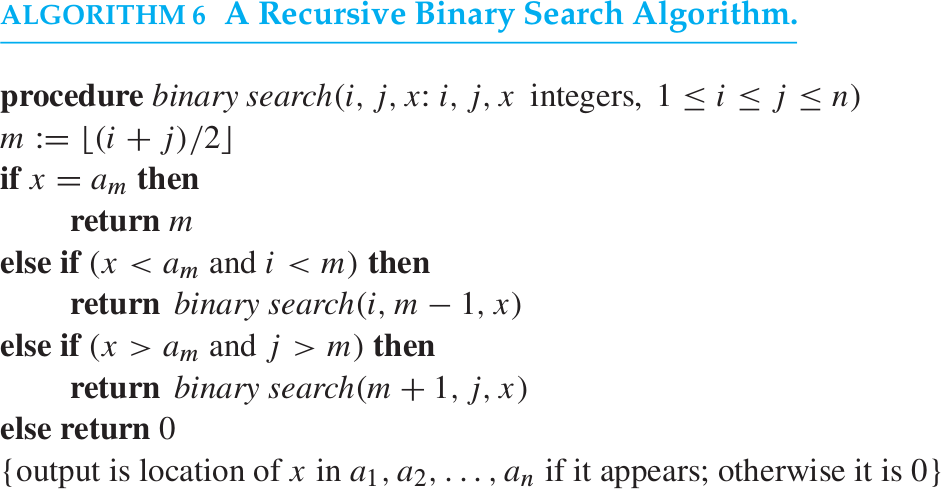
\includegraphics[width=0.8\textwidth]{binary-search-recursive}
\end{center}
\end{frame}

\section{Endurkvæmni og ítrun}

\begin{frame}{Endurkvæmni og ítrun}
\begin{itemize}
 \item Höfum séð endurkvæm reiknirit sem byrja á að skoða heildarmyndina og brjóta hana svo niður í smærri tilvik
 \item Gætum þess í stað séð fyrir okkur að við byrjum á að skoða smáu tilvikin og ``byggjum svo upp'' í þau stóru
 \begin{itemize}
  \item Slíka aðferðafræði köllum við ítrun
  \item Ítrun er venjulega framkvæmd með lykkjum
 \end{itemize}
 \item Ítrun og endurkvæmni framkvæma hliðstæða útreikninga!
\end{itemize}
\end{frame}

\begin{frame}{Endurkvæmni og ítrun}
\begin{itemize}
 \item Hvenær á að nota endurkvæmni og hvenær á að nota ítrun við forritun? \pause
 \begin{itemize}
  \item Ráðlegging undirritaðs: Notið það sem ykkur finnst lýsa vandamálinu best
  \begin{itemize}
   \item Tími forritarans er verðmætur
   \item Getið síðan breytt úr einu í annað ef \emph{mælingar} sýna að upprunalega nálgunin er ekki skilvirk
  \end{itemize}
  \item Þekkið forritunarmálin sem þið eruð að nota - styðja þau endurkvæmni vel?
 \end{itemize}
\end{itemize}
\end{frame}

\begin{frame}{Næst}
\begin{itemize}
    \item Talning og rakningarvensl (8.1)
    \begin{itemize}
        \item Kvik bestun
    \end{itemize}
    \item Lausnir á línulegum rakningarvenslum (8.2)
    \item Deila-og drottna reiknirit (8.3)
\end{itemize}
\end{frame}


\end{document}
